\documentclass[a4paper]{article}
\usepackage[utf8]{inputenc}
\usepackage[a4paper, left=2.5cm, right=2.5cm, top=2cm, bottom=2cm]{geometry}
\usepackage{lmodern}
\usepackage[T1]{fontenc}
\usepackage{graphicx}
\usepackage{amssymb}
\usepackage[utf8]{inputenc}
\usepackage{pgfplots}
\pgfplotsset{width=6cm,compat=1.9}
\usepackage{multicol}
\usepackage{csquotes}
\usepackage{amsfonts}
\usetikzlibrary{angles, quotes}

\newcommand{\overbar}[1]{\mkern 1.5mu\overline{\mkern-1.5mu#1\mkern-1.5mu}\mkern 1.5mu}
\renewcommand{\thesection}{\Alph{section}}
\renewcommand{\thesubsection}{\arabic{subsection}}
\renewcommand{\thesubsubsection}{(\emph{\alph{subsubsection}})}

\title{Nombres complexes}
\author{Hugo Lageneste}
\date{Février 2020}

\begin{document}

{Hugo \textsc{Lageneste}}\\
{Mathématiques - Nombres complexes}

\begin{center}
 \newcommand{\HRule}{\rule{\linewidth}{0.5mm}}
 {\huge \bfseries Nombres complexes}\\[0.1cm]
\end{center}

\section{Nombre complexe}
\subsection{Forme algébrique}
\subsubsection{Définition}
{La forme algébrique de $z$ est notée}
\[z=a+bi\]

\subsubsection{Parties réelle et imaginaire}
{Les parties réelles et imaginaires de $z$ sont $a$ et $b$, notées}
\[Re(z)=a \quad\quad Im(z)=b\]

\subsection{Conjugué}
\subsubsection{Définition}
{Le conjugué de $z$ noté $\bar{z}$ est défini par $\bar{z}=a+bi$}

\subsubsection{Propriétés}
\begin{multicols}{3}
	\begin{itemize}
  		\item{$\bar{z} + z = 2Re(z)$}
  		\item{$\bar{z} - z = 2iIm(z)$}
  		\item{$\overbar{z + z\prime} = \bar{z} + \bar{z\prime}$}
  		\item{$\overbar{zz\prime} = \bar{z} \times \bar{z\prime}$}
  		\item{Si $z\prime$ non nul: $\overbar{\left(\frac{z}{z\prime}\right)} = \frac{\bar{z}}{\bar{z\prime}}$}
  		\item{$\forall n \in \mathbb{Z}$: $\overbar{z^n}=\overbar{z}^n$}
	\end{itemize}
\end{multicols}

\subsection{Module}
\subsubsection{Définition}
{On appelle module de $z$, $|z|$ défini par}
\[|z|=\sqrt{a^2+b^2}\]

\subsubsection{Propriétés}
\begin{multicols}{3}
	\begin{itemize}
  		\item{$z\bar{z}=|z|^2$}
  		\item{$|z|=|\bar{z}|$}
  		\item{$|z|=|-z|$}
  		\item{$|zz\prime| = |z| \times |z|$}
  		\item{Si $z\prime$ non nul: $\left|\frac{z}{z\prime}\right| = \frac{|z|}{\left|z\prime\right|}$}
  		\item{$\forall n \in \mathbb{N}$: $\left|z^n\right|=|z|^n$}
	\end{itemize}
\end{multicols}

\subsection{Représentation}
{Soit un repère orthonormal $\left(O, \overrightarrow{u}; \overrightarrow{v}\right)$}\\
{Le point $M\left(a; b\right)$ a pour affixe $z=a+bi$}\\
{Le vecteur $\overrightarrow{OM}$ a donc pour affixe $z$ et $|z|=OM$}

\section{Équations dans $\mathbb{C}$}
\subsection{Polynômes du second degré}
{Soit $az^2+bz+c=0$ avec $a \neq 0$}

\begin{itemize}
  	\item{Si $\Delta > 0$, il y a deux solutions réelles}
  	\[z=\frac{-b\pm\sqrt{\Delta}}{2a}\]
  	\item{Si $\Delta = 0$, il y a une solution réelle}
  	\[z_0=\frac{-b}{2a}\]
  	\item{Si $\Delta < 0$, il y a deux solutions complexes}
  	\[z=\frac{-b\pm i\sqrt{-\Delta}}{2a}\]
\end{itemize}

\section{Formes trigonométriques et exponentielles}
\subsection{Argument}
{On note $\arg(z)$ la mesure de l'angle orienté $(\overrightarrow{u}; \overrightarrow{OM})$}
\[\arg(z)=(\overrightarrow{u}; \overrightarrow{OM})[2\pi]\]

\begin{center}
	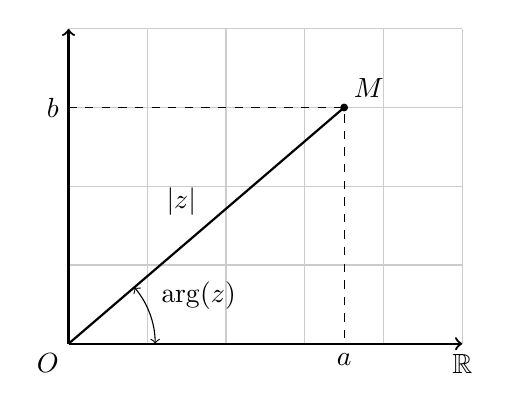
\begin{tikzpicture}
  		\draw[thin,gray!40] (0,0) grid (5,4);
  		\draw[thick, ->] (0,0) -- (5,0) coordinate[label=below: $\mathbb{R}$] (x);
	\draw[thick, ->] (0,0) -- (0,4);
  		\coordinate[label=below left:$ O $] (O);
  		\fill (3.5,3) coordinate[label=above right:$M$] (z) circle(0.05);
		\draw[dashed] (0,3) node[left] {$b$} -| (3.5,0) node[below] {$a$};
		\draw[thick]  (O) to ["$|z|$"] (3.5,3);
		\pic [draw, <->, angle radius=11mm, angle eccentricity=1.6, "$\arg(z)$"] {angle = x--O--z};
	\end{tikzpicture}\\
	\caption{Représentation de l'angle orienté $(\overrightarrow{u}; \overrightarrow{OM})$ et du vecteur $\overrightarrow{OM}$}
\end{figure}

\subsection{Forme trigonométrique}
\subsubsection{Définition}
{Soit $z$ d'argument $\theta$}\\
\[z=|z|\left(\cos(\theta)+i\sin(\theta)\right)\]

\subsubsection{Propriétés}

\begin{center}
	\begin{itemize}
  		\item{$\arg(zz\prime)=\arg(z)+\arg(z\prime)[2\pi]$}
  		\item{$\arg(\frac{1}{z})=-\arg(z)[2\pi]$}
  		\item{$\arg(\frac{z}{z\prime})=\arg(z)-\arg(z\prime)[2\pi]$}
  		\item{$\forall n \in \mathbb{N}$: $\arg(z^n)=n\arg(z)[2\pi]$}
  		\item{$z$ est réel $\Leftrightarrow \arg(z)=0[2\pi]$ ou $\arg(z)=\pi[2\pi]$}
  		\item{$z$ est imaginaire $\Leftrightarrow \arg(z)=\frac{\pi}{2}[2\pi]$ ou $\arg(z)=-\frac{\pi}{2}[2\pi]$}
	\end{itemize}	
\end{center}

\subsection{Forme exponentielle}
\subsubsection{Définition}
{$\forall \theta \in \mathbb{R}$, on pose}
\[e^{i\theta}=\cos(\theta)+i\sin(\theta)\]
{Soit $z$ d'argument $\theta$}
\[z=|z|e^{i\theta}\]

\subsubsection{Propriétés}
\begin{multicols}{2}
	\begin{itemize}
  		\item{$\overbar{e^{i\theta}}=e^{-i\theta}$}
  		\item{$e^{i\left(\theta+\theta\prime\right)}=e^{i\theta}e^{i\theta\prime}$}
  		\item{$\frac{1}{e^{i\theta}}=e^{i\theta}$}
  		\item{$\forall n \in \mathbb{Z}$: $\left(e^{i\theta}\right)^n=e^{in\theta}$}
	\end{itemize}
\end{multicols}

\subsubsection{Formule d'Euler}
{$\forall \theta \in \mathbb{R}$}

\[\cos(\theta)=\frac{e^{i\theta}+e^{-i\theta}}{2} \quad\quad\quad \sin(\theta)=\frac{e^{i\theta}-e^{-i\theta}}{2i}\]

\section{Interprétation géométrique}
\subsection{Distance}
\[AB=\left|z_B-z_A\right|\]
\subsection{Angle}
\[\left(\overrightarrow{u}; \overrightarrow{AB}\right)=\arg(z_B-z_A)[2\pi]\]
\subsection{Argument d'un quotient}
\[\left(\overrightarrow{v_1}; \overrightarrow{v_2}\right)=\arg\left(\frac{z_2}{z_1}\right)\]

\end{document}⏎